\section{Practice: Phân loại ảnh số viết tay 0 và 1}

% ======================================
% Slide 5.1: Giới thiệu bài toán
% ======================================
\begin{frame}{Bài toán: Phân biệt chữ số 0 và 1}
  \begin{itemize}
    \item \textbf{Mục tiêu:} Xây dựng mô hình SVM phân loại ảnh chứa chữ số viết tay \textbf{0} và \textbf{1}.
    \item \textbf{Dữ liệu:} Sử dụng tập MNIST (hoặc phiên bản thu gọn) – ảnh xám kích thước $28 \times 28$ pixels.
    \item \textbf{Vì sao chọn SVM?}
      \begin{itemize}
        \item Dữ liệu nhỏ, số chiều trung bình ($784$).
        \item Ranh giới giữa 0 và 1 gần như tuyến tính khả tách.
        \item SVM hoạt động rất tốt trên bài toán này.
      \end{itemize}
  \end{itemize}
  \centering
  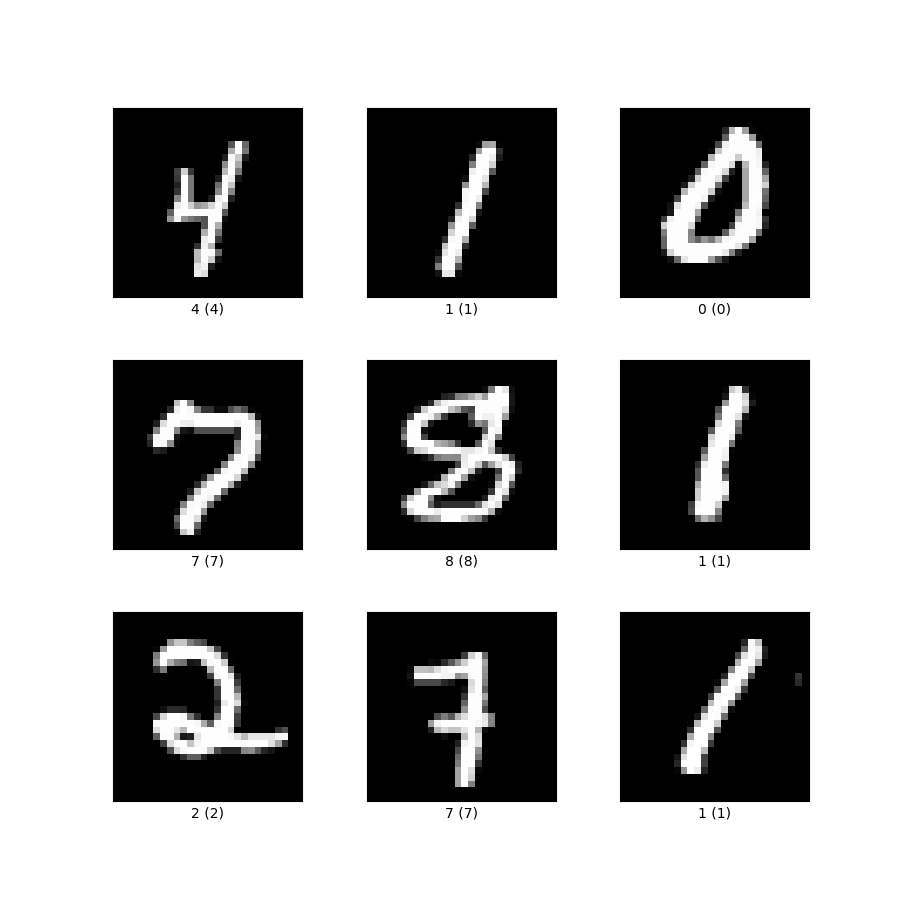
\includegraphics[width=0.25\textwidth]{img/chapter_05/mnist_samples.png}
\end{frame}

% ======================================
% Slide 5.2: Khám phá dữ liệu và tiền xử lý
% ======================================
\begin{frame}[fragile]{Tải dữ liệu và tiền xử lý}
  \begin{block}{Code tải và lọc dữ liệu}
    \begin{semiverbatim}
from sklearn.datasets import fetch_openml
from sklearn.model_selection import train_test_split

mnist = fetch_openml('mnist_784', version=1)
X, y = mnist.data, mnist.target.astype(int)
mask = (y == 0) | (y == 1)
X_bin, y_bin = X[mask], y[mask]
    \end{semiverbatim}
  \end{block}
  \begin{itemize}
    \item \textbf{Phẳng hóa:} Ảnh $28 \times 28$ được duỗi thành vector $784$ chiều.
    \item \textbf{Chuẩn hóa:} Dùng \texttt{StandardScaler} để đưa dữ liệu về phân phối chuẩn.
  \end{itemize}
  \begin{exampleblock}{Lưu ý}
    Với SVM, \textbf{luôn chuẩn hóa} dữ liệu trước khi huấn luyện!
  \end{exampleblock}
\end{frame}

\begin{frame}{EDA: Phân phối nhãn và ảnh trung bình}
  \begin{columns}[T]
    \begin{column}{0.5\textwidth}
      \centering
      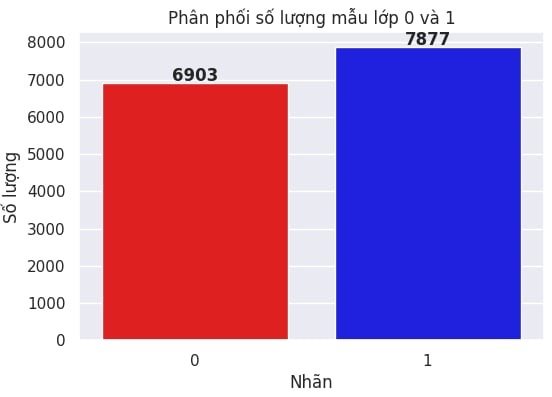
\includegraphics[width=0.7\textwidth, keepaspectratio]{img/chapter_05/label_distribution.jpg}
      \begin{itemize}
        \item Dữ liệu khá cân bằng giữa hai lớp 0 và 1.
        \item Không cần áp dụng kỹ thuật cân bằng lớp.
      \end{itemize}
    \end{column}
    \begin{column}{0.5\textwidth}
      \centering
      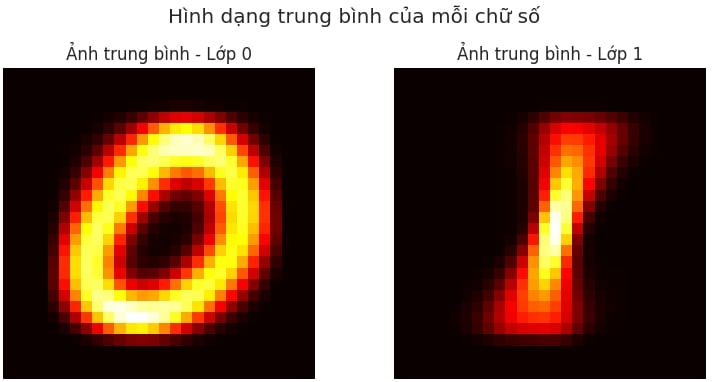
\includegraphics[width=0.7\textwidth, keepaspectratio]{img/chapter_05/average_image.jpg}
      \begin{itemize}
        \item Ảnh trung bình cho thấy sự khác biệt rõ rệt về hình dạng.
        \item Lớp 0 có xu hướng tròn, lớp 1 có nét thẳng đứng.
      \end{itemize}
    \end{column}
  \end{columns}
  \vspace{0.2cm}
  \begin{block}{Nhận xét}
    Hai lớp có đặc trưng trực quan khá khác biệt, gợi ý rằng một mô hình tuyến tính có thể phân tách tốt.
  \end{block}
\end{frame}

\begin{frame}{EDA: Phân bố cường độ pixel}
  \centering
  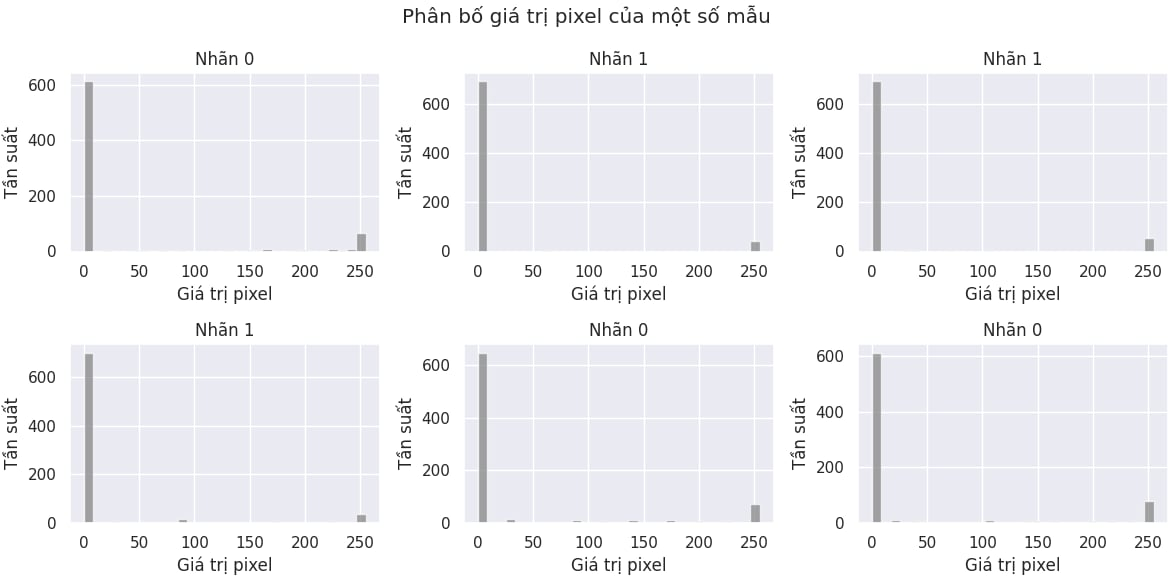
\includegraphics[width=0.7\textwidth, keepaspectratio]{img/chapter_05/pixel_i_distribution.jpg}
  \vspace{0.2cm}
  \begin{itemize}
    \item Biểu đồ histogram cho thấy phần lớn pixel có giá trị thấp (nền tối).
    \item Các pixel sáng tập trung ở vùng chữ viết, tạo nên đặc trưng phân biệt.
    \item \textbf{Chuẩn hóa dữ liệu} (StandardScaler) là cần thiết để SVM không bị ảnh hưởng bởi thang đo.
  \end{itemize}
\end{frame}

% ======================================
% Slide 5.3: Xây dựng mô hình SVM tuyến tính
% ======================================
\begin{frame}[fragile]{Huấn luyện SVM tuyến tính (LinearSVC)}
  \begin{block}{Pipeline đầy đủ}
    \begin{semiverbatim}
from sklearn.pipeline import Pipeline
from sklearn.preprocessing import StandardScaler
from sklearn.svm import LinearSVC

pipeline = Pipeline([
    ('scaler', StandardScaler()),
    ('svm', LinearSVC(C=1.0, max_iter=10000))
])
pipeline.fit(X_train, y_train)
accuracy = pipeline.score(X_test, y_test)
print(f'Accuracy: {accuracy:.4f}')
    \end{semiverbatim}
  \end{block}

\end{frame}

\begin{frame}[fragile]{Huấn luyện SVM tuyến tính (LinearSVC)}
    \begin{itemize}
        \item \textbf{Tham số $C$:} Giữ mặc định $1.0$ (có thể tinh chỉnh sau).
        \item \textbf{max\_iter:} Tăng lên để đảm bảo hội tụ.
    \end{itemize}
\end{frame}
% ======================================
% Slide 5.4: Đánh giá mô hình chi tiết
% ======================================
\begin{frame}{Đánh giá mô hình}
  \begin{columns}
    \begin{column}{0.5\textwidth}
      \textbf{Confusion Matrix}
      \begin{itemize}
        \item True Positive (1 được đoán đúng)
        \item True Negative (0 được đoán đúng)
        \item False Positive / Negative
      \end{itemize}
      \vspace{0.2cm}
      \centering
      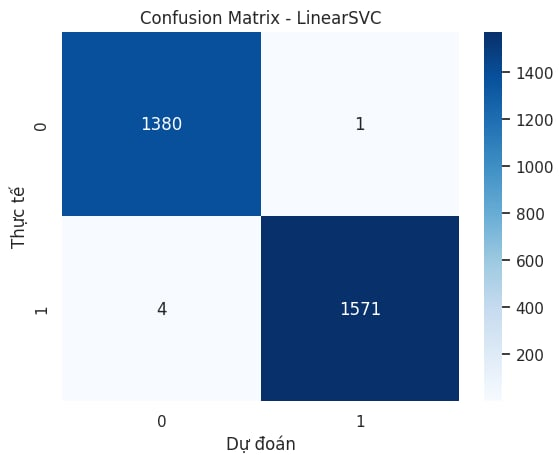
\includegraphics[width=0.8\textwidth]{img/chapter_05/confusion_matrix_linearSVM.jpg}
    \end{column}
    \begin{column}{0.5\textwidth}
      \textbf{Các metric}
      \begin{itemize}
        \item Accuracy: $\frac{TP+TN}{Total}$
        \item Precision: $\frac{TP}{TP+FP}$
        \item Recall: $\frac{TP}{TP+FN}$
        \item F1-score
      \end{itemize}
      \begin{exampleblock}{Kết quả điển hình}
        Với 0 vs 1, accuracy thường đạt \textbf{>99.5\%}.
      \end{exampleblock}
    \end{column}
  \end{columns}
\end{frame}

% ======================================
% Slide 5.5: Trực quan hóa Support Vectors
% ======================================
\begin{frame}{Trực quan hóa Support Vectors}
  \begin{itemize}
    \item Mỗi điểm dữ liệu có hệ số $\alpha_i$. Nếu $\alpha_i > 0$, điểm đó là \textbf{support vector}.
    \item Support vectors nằm trên hoặc trong lề margin, quyết định vị trí siêu phẳng.
    \item Đối với LinearSVC, có thể truy cập thuộc tính \texttt{svm.coef\_} và \texttt{svm.intercept\_}.
  \end{itemize}
  \vspace{0.2cm}
  \begin{block}{Minh họa (sau khi giảm chiều về 2D)}
    \centering
    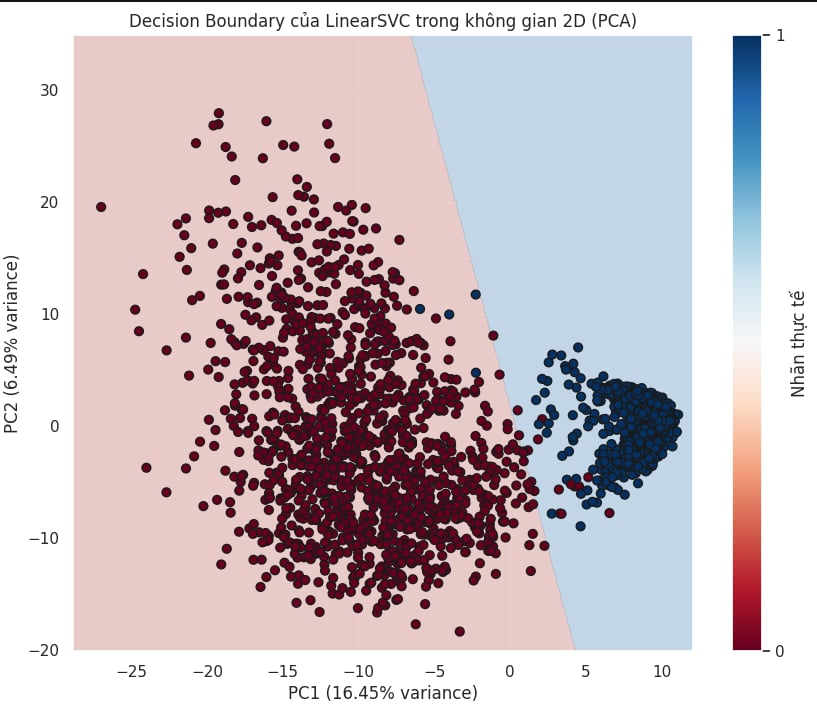
\includegraphics[width=0.45\textwidth]{img/chapter_05/decision_boundary.jpg}
  \end{block}
\end{frame}

% ======================================
% Slide 5.6: So sánh với Kernel RBF
% ======================================
\begin{frame}[fragile]{Thử nghiệm với Kernel RBF}
  \begin{block}{Code so sánh}
    \begin{semiverbatim}
from sklearn.svm import SVC

pipeline_rbf = Pipeline([
    ('scaler', StandardScaler()),
    ('svm', SVC(kernel='rbf', C=1.0, gamma='scale'))
])
pipeline_rbf.fit(X_train, y_train)
print(pipeline_rbf.score(X_test, y_test))
    \end{semiverbatim}
  \end{block}
  \begin{itemize}
    \item Với bài toán 0 vs 1, RBF không cải thiện đáng kể (vẫn ~99.5\%).
    \item \textbf{Thời gian huấn luyện} chậm hơn đáng kể so với LinearSVC.
    \item Kết luận: Chỉ dùng kernel phi tuyến khi thực sự cần thiết.
  \end{itemize}
\end{frame}

% ======================================
% Slide 5.7: Tổng kết và lưu ý thực tế
% ======================================
\begin{frame}{Tổng kết: SVM cho bài toán ảnh}
  \begin{itemize}
    \item \textbf{Quy trình chuẩn:}
      \begin{enumerate}
        \item Flatten ảnh $\rightarrow$ vector.
        \item Chuẩn hóa (StandardScaler).
        \item Chọn mô hình: LinearSVC cho nhanh, SVC+RBF nếu cần phi tuyến.
        \item Đánh giá và tinh chỉnh.
      \end{enumerate}
    \item \textbf{Khi nào dùng SVM cho ảnh?}
      \begin{itemize}
        \item Dữ liệu nhỏ ($n < 10^4$).
        \item Đặc trưng đã được trích xuất tốt (HOG, embeddings).
        \item Cần mô hình giải thích được (support vectors).
      \end{itemize}
    \item \textbf{Hạn chế:}
      \begin{itemize}
        \item Không tận dụng được cấu trúc không gian 2D của ảnh.
        \item Khó mở rộng với ảnh lớn, nhiều lớp.
      \end{itemize}
  \end{itemize}
  \centering
  \textbf{$\rightarrow$ Với ảnh phức tạp, Deep Learning (CNN) là lựa chọn tốt hơn.}
\end{frame}

% ======================================
% Slide kết thúc chương (có thể là Q&A)
% ======================================
\begin{frame}{Q\&A – Thực hành SVM}
  \centering
  \Large
 Arigathanksssss \\
  \vspace{0.5cm}
  \normalsize
\end{frame}